\documentclass[11pt]{article}
\usepackage[left=25mm, right=25mm, top=25mm, bottom=25mm, includehead=true, includefoot=true]{geometry}

\usepackage{graphicx}
\usepackage{url}
\usepackage{natbib} % For referencing
\usepackage{authblk} % For author lists
\usepackage[parfill]{parskip} % Line between paragraphs
\providecommand{\tightlist}{%
  \setlength{\itemsep}{0pt}\setlength{\parskip}{0pt}}

\pagenumbering{gobble} % Turn off page numbers

% Make all headings the same size (11pt):
\usepackage{sectsty}
\sectionfont{\normalsize}
\subsectionfont{\normalsize}
\subsubsectionfont{\normalsize}
\paragraphfont{\normalsize}


\renewcommand{\abstractname}{Summary} % Make 'abstract' be called 'Summary'


% This makes links and bookmarks in the pdf output (should be last usepackage command because it overrides lots of other commands)
\usepackage[pdftex]{hyperref}
\hypersetup{pdfborder={0 0 0} } % This turns off the stupid colourful border around links

\usepackage{framed}
\urlstyle{same}  % don't use monospace font for urls
\usepackage{color}
\usepackage{fancyvrb}
\newcommand{\VerbBar}{|}
\newcommand{\VERB}{\Verb[commandchars=\\\{\}]}
\DefineVerbatimEnvironment{Highlighting}{Verbatim}{commandchars=\\\{\}}
% Add ',fontsize=\small' for more characters per line
\definecolor{shadecolor}{RGB}{248,248,248}
\newenvironment{Shaded}{\begin{snugshade}}{\end{snugshade}}
\newcommand{\KeywordTok}[1]{\textcolor[rgb]{0.13,0.29,0.53}{\textbf{{#1}}}}
\newcommand{\DataTypeTok}[1]{\textcolor[rgb]{0.13,0.29,0.53}{{#1}}}
\newcommand{\DecValTok}[1]{\textcolor[rgb]{0.00,0.00,0.81}{{#1}}}
\newcommand{\BaseNTok}[1]{\textcolor[rgb]{0.00,0.00,0.81}{{#1}}}
\newcommand{\FloatTok}[1]{\textcolor[rgb]{0.00,0.00,0.81}{{#1}}}
\newcommand{\ConstantTok}[1]{\textcolor[rgb]{0.00,0.00,0.00}{{#1}}}
\newcommand{\CharTok}[1]{\textcolor[rgb]{0.31,0.60,0.02}{{#1}}}
\newcommand{\SpecialCharTok}[1]{\textcolor[rgb]{0.00,0.00,0.00}{{#1}}}
\newcommand{\StringTok}[1]{\textcolor[rgb]{0.31,0.60,0.02}{{#1}}}
\newcommand{\VerbatimStringTok}[1]{\textcolor[rgb]{0.31,0.60,0.02}{{#1}}}
\newcommand{\SpecialStringTok}[1]{\textcolor[rgb]{0.31,0.60,0.02}{{#1}}}
\newcommand{\ImportTok}[1]{{#1}}
\newcommand{\CommentTok}[1]{\textcolor[rgb]{0.56,0.35,0.01}{\textit{{#1}}}}
\newcommand{\DocumentationTok}[1]{\textcolor[rgb]{0.56,0.35,0.01}{\textbf{\textit{{#1}}}}}
\newcommand{\AnnotationTok}[1]{\textcolor[rgb]{0.56,0.35,0.01}{\textbf{\textit{{#1}}}}}
\newcommand{\CommentVarTok}[1]{\textcolor[rgb]{0.56,0.35,0.01}{\textbf{\textit{{#1}}}}}
\newcommand{\OtherTok}[1]{\textcolor[rgb]{0.56,0.35,0.01}{{#1}}}
\newcommand{\FunctionTok}[1]{\textcolor[rgb]{0.00,0.00,0.00}{{#1}}}
\newcommand{\VariableTok}[1]{\textcolor[rgb]{0.00,0.00,0.00}{{#1}}}
\newcommand{\ControlFlowTok}[1]{\textcolor[rgb]{0.13,0.29,0.53}{\textbf{{#1}}}}
\newcommand{\OperatorTok}[1]{\textcolor[rgb]{0.81,0.36,0.00}{\textbf{{#1}}}}
\newcommand{\BuiltInTok}[1]{{#1}}
\newcommand{\ExtensionTok}[1]{{#1}}
\newcommand{\PreprocessorTok}[1]{\textcolor[rgb]{0.56,0.35,0.01}{\textit{{#1}}}}
\newcommand{\AttributeTok}[1]{\textcolor[rgb]{0.77,0.63,0.00}{{#1}}}
\newcommand{\RegionMarkerTok}[1]{{#1}}
\newcommand{\InformationTok}[1]{\textcolor[rgb]{0.56,0.35,0.01}{\textbf{\textit{{#1}}}}}
\newcommand{\WarningTok}[1]{\textcolor[rgb]{0.56,0.35,0.01}{\textbf{\textit{{#1}}}}}
\newcommand{\AlertTok}[1]{\textcolor[rgb]{0.94,0.16,0.16}{{#1}}}
\newcommand{\ErrorTok}[1]{\textcolor[rgb]{0.64,0.00,0.00}{\textbf{{#1}}}}
\newcommand{\NormalTok}[1]{{#1}}



% **************  TITLE AND AUTHOR INFORMATION **************

\title{stplanr: A Package for Geographic Transport Data Science}

\author[1]{Robin Lovelace \thanks{r.lovelace@leeds.ac.uk}}
\author[2]{Richard Ellison}
\affil[1]{Institute for Transport Studies, University of Leeds}

\renewcommand\Authands{ and } % correct last comma in author list

\begin{document}

\maketitle

% **************  ABSTRACT/SUMMARY  **************

\begin{abstract}
\centering

Tools for transport planning should be flexible, scalable and
well-integrated with geographic data. \textbf{stplanr} meets each of
these criteria by providing functionality commonly needed for transport
planning in R, with an emphasis on spatial transport data. This includes
tools to import and clean transport datasets; the creation of geographic
`desire lines' from origin-destination data; methods to assign these
desire lines to the transport network, e.g.~via interfaces to routing
services such as CycleStreets.net, Graphhopper and the OpenStreetMap
Routing Machine (OSRM); functions to calculate the geographic attributes
of such routes, such as their bearing and equidistant surroundings; and
`travel watershed' analysis. With reproducible examples and using real
transport datasets, this presentation will demonstrate how R can form
the basis of a reproducible and flexible transport planning workflow. It
concludes with a brief discussion of desirable directions of future
development and ideas about functions for automating the generation of
spatial interaction models.

$ $ \\ {\bf KEYWORDS:} transport planning, geographic data science, software, spatial interaction models.

\end{abstract}

% **************  MAIN BODY OF THE PAPER **************

\section{Introduction}\label{introduction}

Transport planning is a diverse field requiring a wide range of
computational tasks. Software in the transport planner's toolkit should
be flexible, able to handle a wide range of data formats; robust, able
to generate reproducible results for transparent decision-making; and
scalable, able to work at multiple geographic levels from single streets
to large cities and regions.

R can provide a solid basis for a transport planning workflow that meets
each of these criteria.

Inspired by such efforts and driven by our own research needs, our
primary aim for \textbf{stplanr} is to provide an R toolbox for
transport planning (Lovelace and Ellison 2017). Although the focus is on
spatial transport datasets (and most transport problems contain a
spatial component), \textbf{stplanr} also provides functions for
handling non-spatial datasets.

The design of the R language, with its emphasis on flexibility, data
processing and statistical modelling, suggests it can provide a powerful
environment for transport planning research. There are many quantitative
methods in transport planning (Ortúzar and Willumsen 2001) and we have
attempted to focus on those that are most generalisable and frequently
used. \textbf{stplanr} facilitates the following common computational
tasks for transport planning:

\begin{itemize}
\tightlist
\item
  Accessing and processing of data on transport infrastructure and
  behaviour
\item
  Analysis and visualisation of the transport network
\item
  Analysis of origin-destination (OD) data and the visualisation of
  resulting `desire lines'
\item
  The allocation of desire lines to roads and other guideways via
  routing algorithms to show commonly used routes through geographical
  space
\item
  The aggregation of routes to estimate total levels of flow on segments
  throughout the transport network
\item
  Development of models to estimate transport behaviour currently and
  under various scenarios of change
\item
  The calculation of `catchment areas' affected by transport
  infrastructure
\end{itemize}

\section{Package structure and
functionality}\label{package-structure-and-functionality}

The package can be installed and loaded in the usual way (see the
package's \href{https://github.com/ropensci/stplanr}{README} for
dependencies and access to development versions):

\begin{Shaded}
\begin{Highlighting}[]
\KeywordTok{install.packages}\NormalTok{(}\StringTok{"stplanr"}\NormalTok{)}
\end{Highlighting}
\end{Shaded}

\begin{Shaded}
\begin{Highlighting}[]
\KeywordTok{library}\NormalTok{(stplanr)}
\end{Highlighting}
\end{Shaded}

\begin{verbatim}
## Loading required package: sp
\end{verbatim}

As illustrated by the message emitted when \textbf{stplanr} is loaded,
it depends on \textbf{sp}. This means that the spatial data classes
commonly used in the package will work with generic R functions such as
\texttt{summary}, \texttt{aggregate} and, as illustrated in the figures
below, \texttt{plot}.

\subsection{Core functions and
classes}\label{core-functions-and-classes}

The package's core functions are structured around 3 common types of
spatial transport data:

\begin{itemize}
\tightlist
\item
  Origin-destination (OD) data, which report the number of people
  travelling between origin-destination pairs. This type of data is not
  explicitly spatial (OD datasets are usually represented as data
  frames) but represents movement over space between points in
  geographical space. An example is provided in the \texttt{flow}
  dataset.
\item
  Line data, one dimensional linear features on the surface of the
  Earth. These are typically stored as a \texttt{SpatialLinesDataFrame}.
\item
  Route data are special types of lines which have been allocated to the
  transport network. Routes typically result from the allocation of a
  straight `desire line' allocated to the route network with a
  \texttt{route\_} function. Route network represent many overlapping
  routes. All are typically stored as \texttt{SpatialLinesDataFrame}.
\end{itemize}

For ease of use, functions focussed on each data type have been
developed with names prefixed with \texttt{od\_}, \texttt{line\_} and
\texttt{route\_} respectively. Additional `core functions' could be
developed, such as those prefixed with \texttt{rn\_} (for working with
route network data) and \texttt{g\_} functions for geographic operations
such as buffer creation on lat/lon projected data (this function is
currently named \texttt{buff\_geo}). We plan to elicit feedback on such
changes before implementing them.

All functions provided by \textbf{stplanr} can be printed with the
\texttt{lsf.str("package:stplanr",\ all\ =\ TRUE)}.

\subsection{Accessing and processing transport
data}\label{accessing-and-processing-transport-data}

\textbf{stplanr} provides a variety of different functions that
facilitate importing common data formats used for transport analysis
into R. Although transport analysis generally requires some
transport-specific datasets, it also typically relies heavily on common
sources of data including census data as described in the
\href{https://github.com/ropensci/stplanr/blob/master/vignettes/stplanr-paper.Rmd}{package's
vignette}.

\subsection{Creating geographic desire
lines}\label{creating-geographic-desire-lines}

Perhaps the most common type of aggregate-level transport information is
origin-destination (`OD') data. This can be presented either as a matrix
or (more commonly) a long table of OD pairs. An example of this type of
raw data is provided below (see \texttt{?flow} to see how this dataset
was created).

\begin{Shaded}
\begin{Highlighting}[]
\KeywordTok{data}\NormalTok{(}\StringTok{"flow"}\NormalTok{, }\DataTypeTok{package =} \StringTok{"stplanr"}\NormalTok{)}
\KeywordTok{head}\NormalTok{(flow[}\KeywordTok{c}\NormalTok{(}\DecValTok{1}\NormalTok{:}\DecValTok{3}\NormalTok{, }\DecValTok{12}\NormalTok{)])}
\end{Highlighting}
\end{Shaded}

\begin{verbatim}
##        Area.of.residence Area.of.workplace All Bicycle
## 920573         E02002361         E02002361 109       2
## 920575         E02002361         E02002363  38       0
## 920578         E02002361         E02002367  10       0
## 920582         E02002361         E02002371  44       3
## 920587         E02002361         E02002377  34       0
## 920591         E02002361         E02002382   7       0
\end{verbatim}

\begin{Shaded}
\begin{Highlighting}[]
\KeywordTok{data}\NormalTok{(}\StringTok{"cents"}\NormalTok{, }\DataTypeTok{package =} \StringTok{"stplanr"}\NormalTok{)}
\KeywordTok{as.data.frame}\NormalTok{(cents[}\DecValTok{1}\NormalTok{:}\DecValTok{3}\NormalTok{, -}\KeywordTok{c}\NormalTok{(}\DecValTok{3}\NormalTok{,}\DecValTok{4}\NormalTok{)])}
\end{Highlighting}
\end{Shaded}

\begin{verbatim}
##       geo_code  MSOA11NM coords.x1 coords.x2
## 1708 E02002384 Leeds 055 -1.546463  53.80952
## 1712 E02002382 Leeds 053 -1.511861  53.81161
## 1805 E02002393 Leeds 064 -1.524205  53.80410
\end{verbatim}

We use \texttt{od2line} to combine \texttt{flow} and \texttt{cents}, to
join the former to the latter. We will visualise the \texttt{l} object
created below in the next section.

\begin{Shaded}
\begin{Highlighting}[]
\NormalTok{l <-}\StringTok{ }\KeywordTok{od2line}\NormalTok{(}\DataTypeTok{flow =} \NormalTok{flow, }\DataTypeTok{zones =} \NormalTok{cents)}
\end{Highlighting}
\end{Shaded}

The data is now in a form that is much easier to analyse. We can plot
the data with the command \texttt{plot(l)}, which was not possible
before. Because the \texttt{SpatialLinesDataFrame} object also contains
data per line, it also helps with visualisation of the flows, as
illustrated in Figure \ref{fig:lines_routes}.

\subsection{Allocating flows to the transport
network}\label{allocating-flows-to-the-transport-network}

\textbf{stplanr} tackles this issue of the computational intensity of
complex routing algorithms that can scale nationally and globally by
using 3rd party APIs.

This is illustrated below with \texttt{route\_cyclestreet}, which uses
\href{http://www.cyclestreets.net/api/}{CycleStreets.net API}, a routing
service ``by cyclists for cyclists'' that offers a range route
strategies (primarily `fastest', `quietest' and `balanced') that are
based on a detailed analysis of cyclist wayfinding:\footnote{An API key
  is needed for this function to work. This can be requested (or
  purchased for large scale routing) from
  \href{https://www.cyclestreets.net/api/apply/}{cyclestreets.net/api/apply}.
  See \texttt{?route\_cyclestreet} for details. Thanks to Martin
  Lucas-Smith and Simon Nuttall for making this possible.}

\begin{Shaded}
\begin{Highlighting}[]
\NormalTok{route_bl <-}\StringTok{ }\KeywordTok{route_cyclestreet}\NormalTok{(}\DataTypeTok{from =} \StringTok{"Bradford"}\NormalTok{, }\DataTypeTok{to =} \StringTok{"Leeds"}\NormalTok{)}
\NormalTok{route_c1_c2 <-}\StringTok{ }\KeywordTok{route_cyclestreet}\NormalTok{(cents[}\DecValTok{1}\NormalTok{,], cents[}\DecValTok{2}\NormalTok{,])}
\end{Highlighting}
\end{Shaded}

The raw output from routing APIs is usually provided as a JSON or
GeoJSON text string. By default, \texttt{route\_cyclestreet} saves a
number of key variables (including length, time, hilliness and busyness
variables generated by CycleStreets.net) from the attribute data
provided by the API. If the user wants to save the raw output, the
\texttt{save\_raw} argument can be used:

\begin{Shaded}
\begin{Highlighting}[]
\NormalTok{route_bl_raw <-}\StringTok{ }\KeywordTok{route_cyclestreet}\NormalTok{(}\DataTypeTok{from =} \StringTok{"Bradford"}\NormalTok{, }\DataTypeTok{to =} \StringTok{"Leeds"}\NormalTok{, }\DataTypeTok{save_raw =} \OtherTok{TRUE}\NormalTok{)}
\end{Highlighting}
\end{Shaded}

Additional arguments taken by the \texttt{route\_} functions depend on
the routing function in question. By changing the \texttt{plan} argument
of \texttt{route\_cyclestreet} to \texttt{fastest}, \texttt{quietest} or
\texttt{balanced}, for example, routes favouring speed, quietness or a
balance between speed and quietness will be saved, respectively.

To automate the creation of route-allocated lines over many desire
lines, the \texttt{line2route} function loops over each line, wrapping
any \texttt{route\_} function as an input. The output is a
\texttt{SpatialLinesDataFrame} with the same number of dimensions as the
input dataset (see the right panel in Figure \ref{fig:lines_routes}).

\begin{verbatim}
routes_fast <- line2route(l = l, route_fun = route_cyclestreet)
\end{verbatim}

The result of this `batch routing' exercise is illustrated in Figure
\ref{fig:lines_routes}. The red lines in the left hand panel are very
different from the hypothetical straight `desire lines' often used in
transport research, highlighting the importance of this route-allocation
functionality.

\begin{Shaded}
\begin{Highlighting}[]
\KeywordTok{plot}\NormalTok{(route_network, }\DataTypeTok{lwd=}\DecValTok{0}\NormalTok{)}
\KeywordTok{plot}\NormalTok{(l, }\DataTypeTok{lwd =} \NormalTok{l$All /}\StringTok{ }\DecValTok{10}\NormalTok{, }\DataTypeTok{add =} \OtherTok{TRUE}\NormalTok{)}
\KeywordTok{lines}\NormalTok{(routes_fast, }\DataTypeTok{col =} \StringTok{"red"}\NormalTok{)}
\NormalTok{routes_fast$All <-}\StringTok{ }\NormalTok{l$All}
\NormalTok{rnet <-}\StringTok{ }\KeywordTok{overline}\NormalTok{(routes_fast, }\StringTok{"All"}\NormalTok{, }\DataTypeTok{fun =} \NormalTok{sum)}
\NormalTok{rnet$flow <-}\StringTok{ }\NormalTok{rnet$All /}\StringTok{ }\KeywordTok{mean}\NormalTok{(rnet$All) *}\StringTok{ }\DecValTok{3}
\KeywordTok{plot}\NormalTok{(rnet, }\DataTypeTok{lwd =} \NormalTok{rnet$flow /}\StringTok{ }\KeywordTok{mean}\NormalTok{(rnet$flow))}
\end{Highlighting}
\end{Shaded}

\begin{figure}
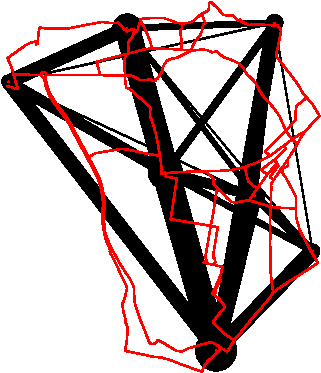
\includegraphics[width=0.5\linewidth]{stplanr-paper_files/figure-latex/lines_routes-1} 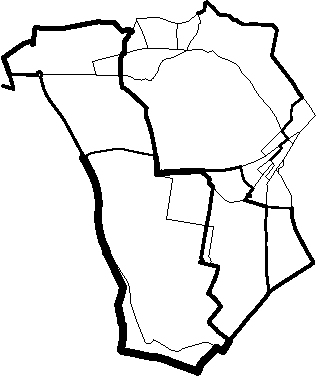
\includegraphics[width=0.5\linewidth]{stplanr-paper_files/figure-latex/lines_routes-2} \caption{Visualisation of travel desire lines, with width proportional to number of trips between origin and destination (black) and routes allocated to network  (red) in the left-hand panel. The right hand panel shows the route network dataset generated by overline().}\label{fig:lines_routes}
\end{figure}

To estimate the amount of capacity needed at each segment on the
transport network, the \texttt{overline} function demonstrated above, is
used to divide line geometries into unique segments and aggregate the
overlapping values. The results, illustrated in the right-hand panel of
Figure \ref{fig:lines_routes}, can be used to estimate where there is
most need to improve the transport network, for example informing the
decision of where to build new bicycle paths.

Additional routing APIs were added with the functions
\texttt{route\_graphhopper}, \texttt{route\_transportapi\_public} and
\texttt{viaroute}. These interface to Graphhopper, TransportAPI and the
Open Source Routing Machine (OSRM) routing services, respectively. The
great advantage of OSRM is that it allows you to run your own routing
services on a local server, greatly increasing the rate of route
generation.

\subsection{Spatial interaction
models}\label{spatial-interaction-models}

With its facilities for generating geographic travel data and native
language of R, which excels in statistical modelling \textbf{stplanr} is
well set-up to be a port of call for spatial interaction (SI) models. A
brief example below shows the implementation of the \emph{radiation
model} in \textbf{stplanr}. Many other SI model forms could be added,
perhaps using a generic function \texttt{si()}:

\begin{Shaded}
\begin{Highlighting}[]
\CommentTok{# load some points data}
\KeywordTok{data}\NormalTok{(cents)}
\CommentTok{# plot the points to check they make sense}
\KeywordTok{plot}\NormalTok{(cents)}
\end{Highlighting}
\end{Shaded}

\begin{figure}
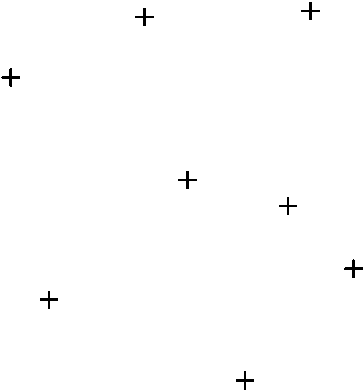
\includegraphics[width=\textwidth]{stplanr-paper_files/figure-latex/unnamed-chunk-8-1} \caption{Results of running a Spatial Interaction model (the radiation model) with stplanr.}\label{fig:unnamed-chunk-81}
\end{figure}

\begin{Shaded}
\begin{Highlighting}[]
\KeywordTok{class}\NormalTok{(cents)}
\end{Highlighting}
\end{Shaded}

\begin{verbatim}
## [1] "SpatialPointsDataFrame"
## attr(,"package")
## [1] "sp"
\end{verbatim}

\begin{Shaded}
\begin{Highlighting}[]
\CommentTok{# Create test population to model flows}
\KeywordTok{set.seed}\NormalTok{(}\DecValTok{2050}\NormalTok{)}
\NormalTok{cents$population <-}\StringTok{ }\KeywordTok{runif}\NormalTok{(}\DataTypeTok{n =} \KeywordTok{nrow}\NormalTok{(cents), }\DataTypeTok{min =} \DecValTok{100}\NormalTok{, }\DataTypeTok{max =} \DecValTok{1000}\NormalTok{)}
\CommentTok{# estimate}
\NormalTok{flowlines_radiation <-}\StringTok{ }\KeywordTok{od_radiation}\NormalTok{(cents, }\DataTypeTok{pop_var =} \StringTok{"population"}\NormalTok{)}
\NormalTok{flowlines_radiation$flow}
\end{Highlighting}
\end{Shaded}

\begin{verbatim}
##  [1]          NA  28.5716171 199.1483930  45.6047446   7.5864754
##  [6]  21.5568487  41.2170441 105.2684494  24.7449354          NA
## [11] 118.5268678  10.1879935   4.3086722  57.4515754 259.3003676
## [16]  15.9131245  44.3764656 293.7173517          NA   9.8773421
## [21]   7.1271190  35.3137167  81.5452128  15.4279029  85.4088485
## [26]   5.9374332   8.8651941          NA  84.9504273  35.9825242
## [31]  26.8695174  53.6173692   1.8104829   1.2293437   0.7982433
## [36]  84.9504273          NA  19.6809596   2.7914752   1.2033517
## [41]  27.3885572 106.4446453  44.4324793  34.6086394 100.2158728
## [46]          NA 220.5555702  36.7618461  13.8249960 259.3003676
## [51]  59.2543662   6.1879080   3.8213690  34.8945124          NA
## [56]  22.4008006  10.4091206   4.4967751   1.7164989   1.3797507
## [61]   4.7760711   2.0211245 102.2283795          NA
\end{verbatim}

\begin{Shaded}
\begin{Highlighting}[]
\KeywordTok{sum}\NormalTok{(flowlines_radiation$flow, }\DataTypeTok{na.rm =} \OtherTok{TRUE}\NormalTok{) }\CommentTok{# the total flow in the system}
\end{Highlighting}
\end{Shaded}

\begin{verbatim}
## [1] 2937.987
\end{verbatim}

\begin{Shaded}
\begin{Highlighting}[]
\KeywordTok{sum}\NormalTok{(cents$population) }\CommentTok{# the total inter-zonal flow}
\end{Highlighting}
\end{Shaded}

\begin{verbatim}
## [1] 3450.191
\end{verbatim}

\begin{Shaded}
\begin{Highlighting}[]
\KeywordTok{plot}\NormalTok{(flowlines_radiation, }\DataTypeTok{lwd =} \NormalTok{flowlines_radiation$flow /}\StringTok{ }\DecValTok{100}\NormalTok{)}
\KeywordTok{points}\NormalTok{(cents, }\DataTypeTok{cex =} \NormalTok{cents$population /}\StringTok{ }\DecValTok{100}\NormalTok{)}
\end{Highlighting}
\end{Shaded}

\begin{figure}
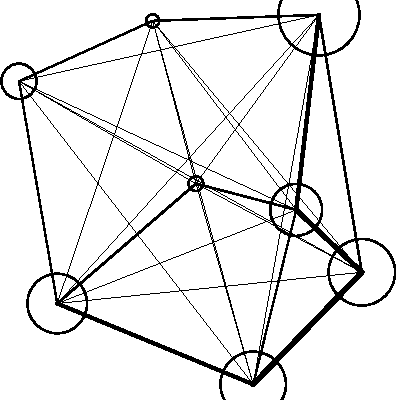
\includegraphics[width=\textwidth]{stplanr-paper_files/figure-latex/unnamed-chunk-8-2} \caption{Results of running a Spatial Interaction model (the radiation model) with stplanr.}\label{fig:unnamed-chunk-82}
\end{figure}

The results show how packaging-up code into peer-reviewed, publicly
accessible software, can enable the reproduction of results in the
emerging field of transport data science. \textbf{stplanr}'s use in the
DfT-funding Propensity to Cycle Tool (PCT) shows that software
development can greatly assist with applied work (Lovelace et al. 2016).

The wider question is: what are the most desirable next steps (or cycle
pedals) forward?

\subsection{Next steps}\label{next-steps}

The next step with \textbf{stplanr} is consolidation. Before moving to
Version \texttt{1.0} we would like to update function names and
behaviour based on first principles. Key to this will be user engagement
and community collaboration so we will encourage this through
`hackathons', on-line demos, documentation, blogs and conferences such
as GISRUK 2017, where this paper was presented.

\subsection*{References}\label{references}
\addcontentsline{toc}{subsection}{References}

\hypertarget{refs}{}
\hypertarget{ref-lovelace_stplanr:_2017}{}
Lovelace, Robin, and Richard Ellison. 2017. ``Stplanr: A Package for
Transport Planning.'' \emph{Under Review}.
\url{https://github.com/ropensci/stplanr}.

\hypertarget{ref-lovelace_propensity_2016}{}
Lovelace, Robin, Anna Goodman, Rachel Aldred, Nikolai Berkoff, Ali
Abbas, and James Woodcock. 2016. ``The Propensity to Cycle Tool: An Open
Source Online System for Sustainable Transport Planning.'' \emph{Journal
of Transport and Land Use} 10 (1).
doi:\href{https://doi.org/10.5198/jtlu.2016.862}{10.5198/jtlu.2016.862}.

\hypertarget{ref-ortuzar_modelling_2001}{}
Ortúzar, Juan de Dios, and Luis G. Willumsen. 2001. \emph{Modelling
Transport}. John Wiley; Sons.


\end{document}